\section{Recasting Examples for Specific Searches}
\label{sec:ch5-recastExamples}

Here we provide examples of recasting specific experimental
searches for several LLP signatures: searches for heavy stable charge particles (HSCPs), displaced
leptons, displaced jets, displaced lepton-jets (LJs), non-pointing photons, and displaced vertices (DV).
These recasting attempts have been made outside the experimental collaborations,
making use of the public information provided by the experimental note or
publication. The aim here is to highlight the challenges faced when recasting
LLP searches and also to highlight the cases where the
experimental information provided is straightforward and useful for
recasting.

\subsection{Heavy Stable Charged Particles (HSCPs)}
\label{sec:ch5-HSCPs}

% JH
\renewcommand{\vec}[1]{\boldsymbol{#1}}
%

Searches for HSCPs are based on the signature
of highly ionizing tracks and/or an anomalous time-of-flight between 
the particle's production at the interaction point and its arrival in the
muon detector~\cite{Fairbairn:2006gg} (see Sec.~\ref{subsec:ExpHSCP} for more details).
Both signatures are sensitive to the particle's velocity and exploit the
production of HSCPs outside of the ultra-relativistic regime,
allowing for a powerful discrimination against the highly boosted Standard Model backgrounds.
HSCP searches assume particles are sufficiently long-lived  to traverse
the entire detector.
% They have been performed at the 7~\cite{Chatrchyan:2012sp,Aad:2012pra},
% 8~\cite{Chatrchyan:2013oca,ATLAS:2014fka} and 13\,TeV
% LHC~\cite{Aaboud:2016dgf,CMS:2016ybj} and interpreted for HSCPs that are
% purely electrically charged or colored, the latter of which hadronize to form
% $R$-hadrons~\cite{Farrar:1978xj}.
They have been interpreted for HSCPs that are 
purely electrically charged or carry color charge, the latter of which hadronize to form
$R$-hadrons as they propagate through the detector~\cite{Farrar:1978xj}.
Typically, the HSCP signature yields high sensitivities providing
a very strong background rejection while still allowing for large
signal efficiencies.
As a consequence, search strategies for new physics models with HSCPs
typically do not benefit from more model-dependent selection criteria, like requiring additional
particles in the event~\cite{Heisig:2012zq}. The corresponding searches can, hence, be
performed in a mostly inclusive manner concentrating on the HSCP candidate itself.
This fact opens up the possibility of providing a widely applicable recasting based on signature
efficiencies. This approach has been followed by the CMS
Collaboration~\cite{Khachatryan:2015lla},
which has provided probabilities for HSCP candidates to pass the on- and
off-line selection criteria for the 8\,TeV LHC run as a function of the relevant kinematical parameters.


In this section we describe the recasting of the 8\,TeV CMS
search for HSCPs and discuss its validation and applicability.
Furthermore, we comment on the attempt to extrapolate
the 8\,TeV signature efficiencies to the corresponding 13\,TeV analysis, for
which the corresponding efficiencies have not been provided by CMS\@.


\subsubsection{Recasting using signature efficiencies}\label{sec:signatureeff}

Ref.~\cite{Khachatryan:2015lla} provides efficiencies for the reconstruction
and selection of HSCP candidates with $|Q|=1$ in the form of on- and
off-line probabilities, $P_\text{on}(\vec{k})$ and $P_\text{off}(\vec{k})$.
These are given as a function of the truth-level kinematics
velocity ($\beta$), pseudo-rapidity ($\eta$) and
transverse momentum ($p_\text{T}$) of isolated HSCP candidates, so
the vector $\vec{k}$ is defined as: $\vec{k}=(\beta,\eta,p_\text{T})$.
The on- and off-line probabilities must be applied to
isolated HSCP candidates, which are required to fulfill
%
\begin{equation}
\left( \sum_{i}^{\stackrel{\text{charged}}{\Delta R<0.3}} \!p_\text{T}^{i}
\right)  < 50\,\text{GeV}
\;,\quad
\left(
\sum_{i}^{\stackrel{\text{visible}}{\Delta R<0.3}}  \frac{E^i}{
|\vec{p}|} \right)  < 0.3\,,
\label{eq:GenTkIso1}
\end{equation}
%
where the sums include all charged and visible particles, respectively,
within a radius of $\Delta R=\sqrt{\Delta\eta^2+\Delta \phi^2}<0.3$ around the
HSCP candidate track, $p_\text{T}^{i}$ denotes their transverse momenta and $E^i$
their energy. Muons are not counted as visible particles and the HSCP itself
is not included in either sum.


If an event contains one or more HSCPs satisfying the above isolation
criteria, the efficiency for the event to pass the analysis selection is
given by:
%
\begin{equation}
\label{eq:Technique}
\epsilon = \epsilon_{\text{on}} \times \epsilon_{\text{off}}
\,.
\end{equation}
%
For an event with one HSCP candidate $\epsilon_{\text{on/off}}$ is
directly given by the signature efficiencies $P_{\text{on/off}}(\vec{k})$.
For an event with two candidates, the efficiency reads~\cite{Khachatryan:2015lla}
\begin{equation}
\label{eq:EventAcceptance}
\epsilon_{\text{on}/\text{off}}
= P_{\text{on}/\text{off}}(\vec{k}^1)  + P_{\text{on}/\text{off}}(\vec{k}^2)
- P_{\text{on}/\text{off}}(\vec{k}^1)  P_{\text{on}/\text{off}}(\vec{k}^2)  \,,
\end{equation}
where $\vec{k}^{1,2}$ are the kinematical vectors of the two HSCPs in the given
event. Therefore the on- and off-line probabilities combined with the isolation
criteria allow for the complete recasting of the HSCP search using only truth-level events generated
in MC.


The recasting of the 8\,TeV search was performed in Ref.~\cite{Heisig:2015yla}
using the procedure described above.
Events were simulated using \textsc{Pythia}~6~\cite{Sjostrand:2006za} and
the total signal efficiency for a given model was then computed using:
%
\begin{equation*}
\epsilon = \frac{1}{N} \sum_{i=1}^{N} \epsilon_i\,.
\end{equation*}
%
where the sum runs over all the ($N$) generated events and $\epsilon_i$ is the
efficiency for each event computed using Eq.~\eqref{eq:Technique}.
Since the probabilities $P_{\text{on/off}}(\vec{k})$ are given for
four distinct cuts on the reconstructed HSCP mass ($m_\text{rec}$),
these were considered as four different signal regions.
The number of observed events and the expected background for which
of these cuts are reported in Ref.~\cite{Khachatryan:2015lla}.


%----------------------------------------------------------------------------------------------------------------
\subsubsection{Validation and applicability}
\label{sec:ch5-validate}
%----------------------------------------------------------------------------------------------------------------

A validation of the method described above was
done in Ref.~\cite{Heisig:2015yla} using the same gauge-mediated supersymmetry
breaking (GMSB) model considered by CMS~\cite{Khachatryan:2015lla}.
This supersymmetric model features a gravitino and a long-lived stau as the lightest and next-to-lightest
supersymmetric particle, respectively.
Since the stau only decays outside the detector volume, all
cascade decays of the produced sparticles terminate in the lightest stau,
which provides the HSCP signature.
The left pane of Fig.~\ref{fig:gmsbComp} compares the
resulting signal efficiency
obtained by the recasting and the full CMS detector
simulation. The signal efficiencies agree within 3\%, demonstrating
that the recast is an excellent approximation to the full CMS simulation. 
The differences are of the order of
the statistical uncertainties from the MC simulation of the signal.
In the right pane of Fig.~\ref{fig:gmsbComp}, we show the 95\% CL upper
limits on the inclusive production cross sections, which, again, agree
(within $\sim 3\%$) with the ones obtained by the full simulation in
Ref.~\cite{Khachatryan:2015lla}.
Note that both limits are based on the discrete mass cuts on $m_\text{rec}$ mentioned
above. In the full CMS analysis~\cite{Chatrchyan:2013oca}, an event-based
mass cut is used, resulting in slightly stronger constraints for some HSCP masses.

%=====================
%    \                                           |
%      \                                         |
%        \                                       |
\begin{figure}[!h]
\centering
\setlength{\unitlength}{1\textwidth}
\begin{picture}(1,0.45)
 \put(0.003,-0.003){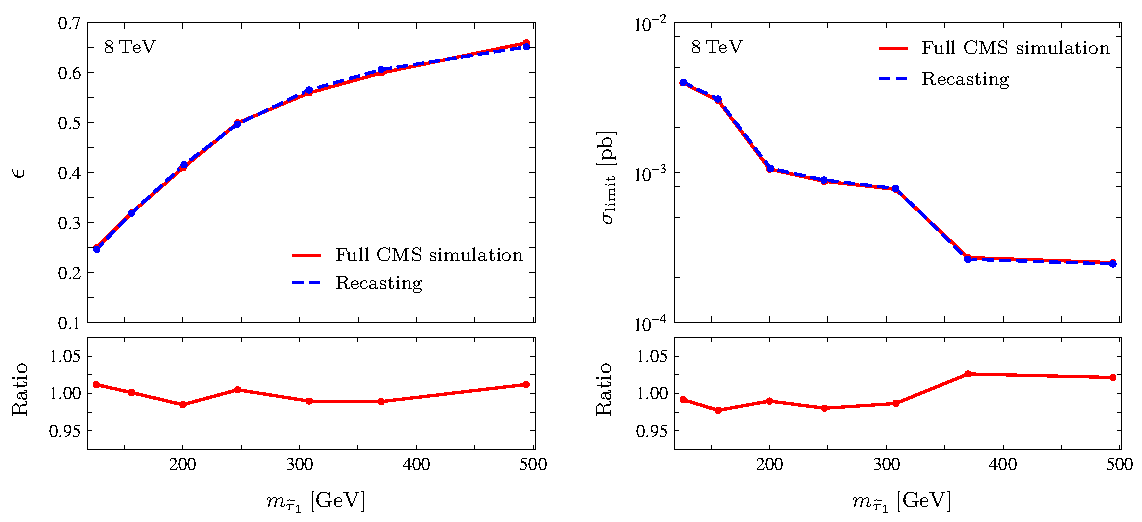
\includegraphics[width=0.99\textwidth]{ch5-figures/HSCP_validation.pdf}}
\end{picture}
\caption{
{\bf{Left: }}Signal efficiency $\epsilon$ of the HSCP search. {\bf{Right: }}95\% CL cross section upper limit
for the GMSB model as the function of the stau mass.
We compare the CMS analysis~\cite{Khachatryan:2015lla}
from the full detector simulation (red solid
lines) with the recasting using signature efficiencies (blue dashed lines).
In the lower frames we show the respective ratios
$\epsilon^\text{Full}/\epsilon^\text{Recast}$,
$\sigma^\text{Full}_\text{limit}/\sigma_\text{limit}^\text{Recast}$.
Taken from Ref.~\cite{Heisig:2015yla}.
}
\label{fig:gmsbComp}
\end{figure}
%                                      \         |
%                                        \       |s
%                                          \     |
%=====================


Due to the inclusive nature of the search, the above recasting provides
a widely applicable and highly reliable way to reinterpret the HSCP search for arbitrary
models containing detector-stable HSCPs. Accordingly it has been used
in a variety of phenomenological studies. For instance,
it has been used for reinterpretations of
supersymmetric models~\cite{Evans:2016zau,Bagnaschi:2016afc,Heisig:2017lik,Liu:2015bma} and
non-supersymmetric models of very weakly interacting dark matter~\cite{Hessler:2016kwm, Garny:2017rxs}.
In Refs.~\cite{Garny:2017rxs,Liu:2015bma}, the recasting has been used to re-interpret the HSCP search
for finite lifetimes by convolving the signature efficiency with the fraction of HSCPs
that decay after traversing the relevant parts of the detector.
The recasting has also been used for a reinterpretation
in terms of simplified models, as discussed in Sec.~\ref{sec:ch5-smsHSCP}.


%----------------------------------------------------------------------------------------------------------------
\subsubsection{Extrapolation to 13\,TeV} \label{sec:extra}
%----------------------------------------------------------------------------------------------------------------

While the CMS search for HSCPs at 8\,TeV has provided the
signature efficiencies discussed above, the same is not true for
the  13\,TeV analysis~\cite{CMS:2016ybj}.
Therefore a straightforward recasting of the Run-2 search is not possible.
Nonetheless, since the 8\,TeV CMS search has proven to be extremely useful
in constraining models with long-lived charged particles,
it would be desirable to recast the 13\,TeV analysis as well.
In the following we discuss an attempt~\cite{LesHouches2017}
to obtain a similar recasting for the corresponding HSCP search at 13\,TeV.
Our aim is to extrapolate the public 8\,TeV efficiencies to the 13\,TeV run by
introducing a correction function $F$ that accounts for the differences between both runs:
\begin{equation}
\label{eq:introF}
P^{13\,\text{TeV}}_{\text{off}}(\vec{k}) = F(\beta) \times
P^{8\,\text{TeV}}_{\text{off}}(\vec{k})\,,
\end{equation}
where we have assumed that the correction function is mainly dependent on the
HSCP velocity. If $F(\beta)$ is sufficient to account for the difference
between both runs and can be computed, we can directly obtain
$P^{13\,\text{TeV}}_{\text{off}}$ and, using the procedure described in
Sec.~\ref{sec:signatureeff}, recast the 13\,TeV analysis.


In order to compute the correction function $F(\beta)$, we use
the total signal efficiencies reported by the
13\,TeV CMS analysis~\cite{CMS:2016ybj} for
direct production of long-lived staus.
Since the signal efficiencies have been provided for six distinct
values of the stau mass, we perform a fit of $F$ to the efficiencies reported.
We chose to parametrize the correction function $F(\beta)$  by eight parameters
($C_{i}$).
Using  {\sc MadGraph5\_aMC@NLO}~\cite{Alwall:2014hca}
and  \textsc{Pythia}~6~\cite{Sjostrand:2006za}, we obtain generator-level events
for each of the stau mass points at $13\,$TeV.
Then, comparing the total signal efficiencies obtained for a given set $C_{i}$
to the efficiencies reported in Ref.~\cite{CMS:2016ybj}, we can determine
the best-fit values for the $C_{i}$ parameters and consequently the
best-fit for the correction function ($F_\text{best-fit}$).
The result of the best-fit function and its $1\sigma$ uncertatinty is shown in
Fig.~\ref{fig:F}. The deviation of $F$ from 1 implies a decrease or increase
of the respective detector and signal efficiency between the 8 and 13\,TeV
analyses.  Fig.~\ref{fig:F} also shows that the function is loosely constrained
for low values of $\beta$.


%=====================
%    \                                           |
%      \                                         |
%        \                                       |
\begin{figure}[t]
\centering
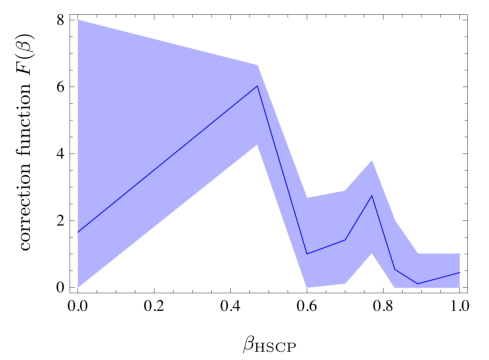
\includegraphics[width=0.7\textwidth]{ch5-figures/HSCP_13TeV_fitB.pdf}
\caption{Best-fit correction function $F(\beta)$ and its $ \pm 1\sigma$ band.
}
\label{fig:F}
\end{figure}
%                                      \         |
%                                        \       |
%                                          \     |
%=====================


In order to verify the validity of the extrapolation to 13\,TeV,
we use $F_\text{best-fit}$ and Eq.~\eqref{eq:introF} to compute the total signal
efficiencies for the same six benchmark points used in the fit. A comparison
between the results obtained through recasting and the efficiencies reported by
CMS is shown by the second and third columns in Table~\ref{tab:eff}.
The results reproduce the CMS values well within the expected uncertainties,
thus validating the fitting procedure.
Furthermore, the inclusion of the correction function significantly improves the
agreement with respect to the direct extrapolation of the 8\,TeV
efficiencies ($F=1$), as shown by the forth column in Table~\ref{tab:eff}.



\begin{table}[t]
\footnotesize
 \begin{center}
\begin{tabular}{c|ccc}
 & \multicolumn{3}{c}{direct production } \\
$m_\text{HSCP}$ [{\rm GeV}] & \,$\epsilon(\text{CMS})$ & $\epsilon(F_\text{best-fit})$& $\epsilon(F=1)$ \\
\hline
200   & \,0.235 & 0.232 & 0.259  \\
308   & \,0.294 & 0.298  & 0.346  \\
494    & \,0.387 & 0.384  & 0.452  \\
651  & \,0.450  & 0.448   & 0.503 \\
1029 & \,0.497 & 0.501  & 0.466 \\
1599 & \,0.428 & 0.429  & 0.225  \\
\hline
\end{tabular}
\end{center}
\caption{Efficiencies for the 13\,TeV LHC for the six benchmark masses in the direct stau production scenario
reported by CMS (second column) and obtained through recasting using
$F_\text{best-fit}$ and without the inclusion of the correction function ($F=1$).}
\label{tab:eff}
\end{table}

The high level of agreement obtained with $F_\text{best-fit}$
for the direct stau benchmark points is expected, since these points
were used in order to fit the correction function.
Therefore an independent test of the above fit
must be performed in order to properly validate the recasting of
the 13\,TeV analysis.
Fortunately CMS has also reported efficiencies for a second scenario,
the GMSB model with long lived staus. This scenario not
only contains direct stau production, but also includes production
through cascade decays of heavier sparticles.
Since the GMSB model produces distinct event topologies, it
provides a good test for the validity of the recasting
procedure.

The results for the six GMSB bechmark points considered in
Ref.~\cite{CMS:2016ybj} are shown in Table~\ref{tab:effGMSB}. As we can
see, they deviate from the CMS values by up to 20\% for large
stau masses, where our estimate undershoots the CMS efficiencies.
Although the overall agreement is improved by the correction function,
the result is not entirely satisfactory, given that
the uncertainties for the 8\,TeV recasting were
under 5\% (see Fig.~\ref{fig:gmsbComp}).
The observed difference might arise from several shortcomings in our description.
In particular, we assume $F$ to only dependent on $\beta$ whereas the full
probability maps are parametrized in the three kinematic variables $\beta, \eta$ and $p_\text{T}$.
However assuming a dependence of all three kinematic variables is clearly
not feasible given the very limited amount of information provided by the
13\,TeV CMS analysis.
Therefore we conclude that it is not possible
to extrapolate the 8\,TeV efficiencies in a straighforward way without
additional information from the experimental collaboration.

\begin{table}[t]
\footnotesize
\begin{center}
\begin{tabular}{c|ccc}
 & \multicolumn{3}{c}{ GMSB } \\
$m_\text{HSCP}$ [{\rm GeV}] & \,$\epsilon(\text{CMS})$ & $\epsilon(F_\text{best-fit})$& $\epsilon(F=1)$ \\
\hline
200     &\,0.276   & 0.297  & 0.279 \\
308   & \, 0.429 &  0.401 & 0.423  \\
494    & \,0.569 & 0.494 & 0.556  \\
651  &  \,0.628 & 0.524 & 0.580 \\
1029 &\,0.665  & 0.538  & 0.493\\
1599 &  \,0.481  & 0.442  & 0.228 \\
\hline
\end{tabular}
\end{center}
\caption{Efficiencies for the 13\,TeV LHC for the six GMSB model benchmark
points reported by CMS (second column)
and obtained through recasting using $F_\text{best-fit}$ and without the inclusion of the correction function ($F=1$).}
\label{tab:effGMSB}
\end{table}


\vskip 0.1in
\noindent {\bf Lessons learned}
\vskip 0.1in
The prominent signature of HSCPs allows for a mostly inclusive search strategy concentrating
on the HSCP track itself. Hence, searches for HSCPs can be re-interpreted using signature
efficiencies in a widely applicable and highly reliable way. This possibility has been followed
by the CMS Collaboration providing signature
efficiency maps for the 8\,TeV LHC\@. The validation reveals an excellent performance. The
recast has been successfully used in the literature.
The signature efficiencies for 8\,TeV can also be used to estimate the ones for the 13\,TeV run by applying
a multiplicative correction function. While such an extrapolation introduces some level of approximation,
a better knowledge of the underlying changes between both runs might reduce the uncertainties.

%% ################################################ %%

\subsection{Displaced Leptons}
\label{sec:ch5-displacedLeptons}

Searching for displaced leptons by requiring the leptons to have large impact parameters with respect to the primary vertex
 is a very clean strategy due to the low backgrounds, and such searches are usually very straightforward to recast.
The CMS displaced $e\mu$ search~\cite{Khachatryan:2014mea} demands two
oppositely charged, different flavour ($e ,\mu$) leptons with large impact
parameters (see also Sec.~\ref{subsec:dleptons}). The recast is fairly straightforward to do, and the biggest difficulty
in doing so is locating all of the relevant information as it is not all
provided within the main document. The ``standard'' isolation requirements used
in the search can be found in an earlier version of the
search~\cite{CMS:2014bra}.
The necessary cuts on the displaced decay position ($v_{T},v_{Z}$) as well as
the selection (as a function of $p_T$), reconstruction (as a function
of impact parameter, $d_0$) and trigger efficiencies can be found on an
additional website~\cite{CMSemuEfficiency} containing auxiliary information for
recasting.  Although all of this information is excellent and greatly
facilitates recasting the search, it is a challenge to collect the relevant information
due to the fact that the additional material is not
referenced in the document.

\begin{table}[t]%
\centering
\parbox{0.4\textwidth}{
\begin{footnotesize}
\begin{tabular}{| c |} \hline
{\bf Cut Summary of CMS displaced $e\mu$}    \\ \hline \hline
{\bf Preselection}    \\ \hline
{1 OS $e^\pm\mu^\mp$ pair} \\
{$|d_0|_\ell>100\,\mu$m} \\
{$p_{T,\ell}>25$ GeV,  $ \left\vert \eta_\ell \right\vert <2.5$} \\
{Reject $1.44 <  \left\vert \eta_e \right\vert<1.56$} \\
{$I^{calo,e}_{\Delta R<0.3}<0.10$}, {$I^{calo,\mu}_{\Delta R<0.4}<0.12$} \\
{ $\Delta R_{\ell j}>0.5\; \forall$ jets with $p_T>10$ GeV } \\
{$\Delta R_{e\mu}>0.5$} \\
{$v_{T,\tilde \ell} < 4 \,\mbox{cm}$, $ v_{Z,\tilde \ell} <  30 \,\mbox{cm}$}\\
{Veto additional leptons} \\
 \hline
\end{tabular}
\end{footnotesize}
% \label{tab:cuts}
}
\qquad
\begin{minipage}[c]{0.45\textwidth}%
\centering
    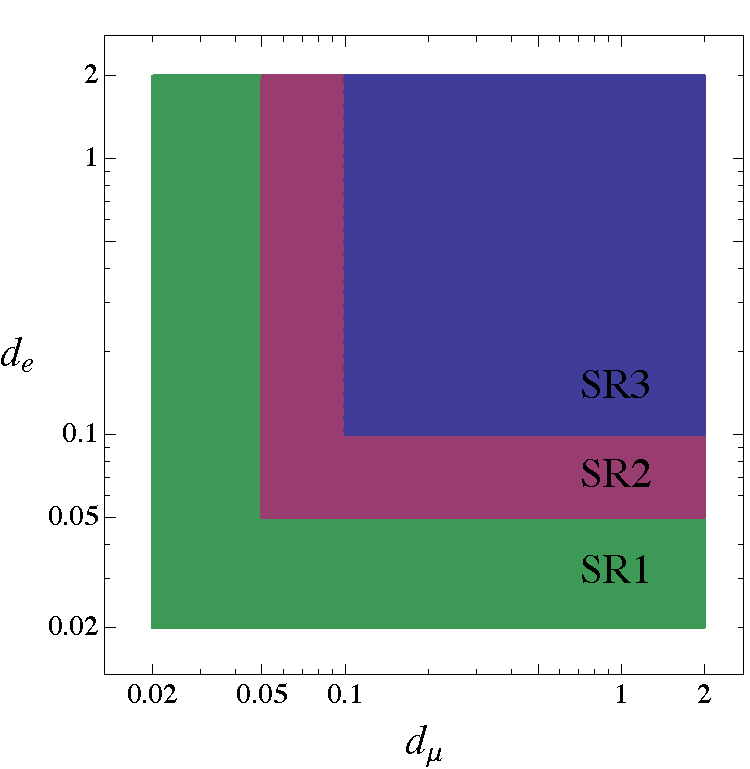
\includegraphics[width=0.9\textwidth,angle=0]{ch5-figures/SRplot.pdf}
\label{tab:cuts}

\end{minipage}
\caption{{\bf Left:} Preselection cuts in Ref.~\cite{Khachatryan:2014mea} (see also \cite{CMS:2014bra,CMSemuEfficiency}).  {\bf Right:} the transverse impact parameter bins that define the exclusive signal regions.  Table and figure taken from Ref.~\cite{Evans:2016zau}.
  \label{tab:cuts}}
\end{table}

\vspace{0.5cm}

The benchmark model used in this search is the direct pair production of stops
that decay through small lepton-flavor-universal RPV $\lambda'_{ijk}L_iQ_jD^c_k$
couplings ($\lambda'_{133}=\lambda'_{233}=\lambda'_{333}$) to yield displaced
$\tilde t \to e b$, $\mu b$, and $\tau b$ decays.  The signal is simple to
generate, where the only challenge is in handling the displacement properly. The most
identifying pre-selection requirement of this search is that the transverse
impact parameter, $|d_0|$, is required to be larger than 100 $\mu$m for both the
electron and muon.  The impact parameter is not the point where the parent
object (e.g., $\tau$ or $b$) decays, \emph{i.e.,} the $v$ mentioned above, 
but rather the
distance to the point of closest approach of the lepton's track relative to the
center of the beampipe in the transverse plane.  Backgrounds in this search from $Z\to\tau\tau$ or heavy
flavor tend to result in leptons that are nearly collinear with the parent due
to the small mass-to-momentum ratio, and yield a small impact parameter even for
decays well on the lifetime tail of the parent.  Events are binned across three
exclusive signal regions: SR3, where both leptons have transverse impact
parameters $|d_0|$ between $0.1$ and $2.0$ cm; SR2, with $|d_0|$ of both
leptons between $0.05$ and $2.0$ cm, but not satisfying the requirement of SR3;
and SR1, with $|d_0|$ between $0.02$ and $2.0$ cm, but not within SR2
or SR3.  All selection requirements are summarized in Table~\ref{tab:cuts}.

\begin{figure}[t]
\begin{center}
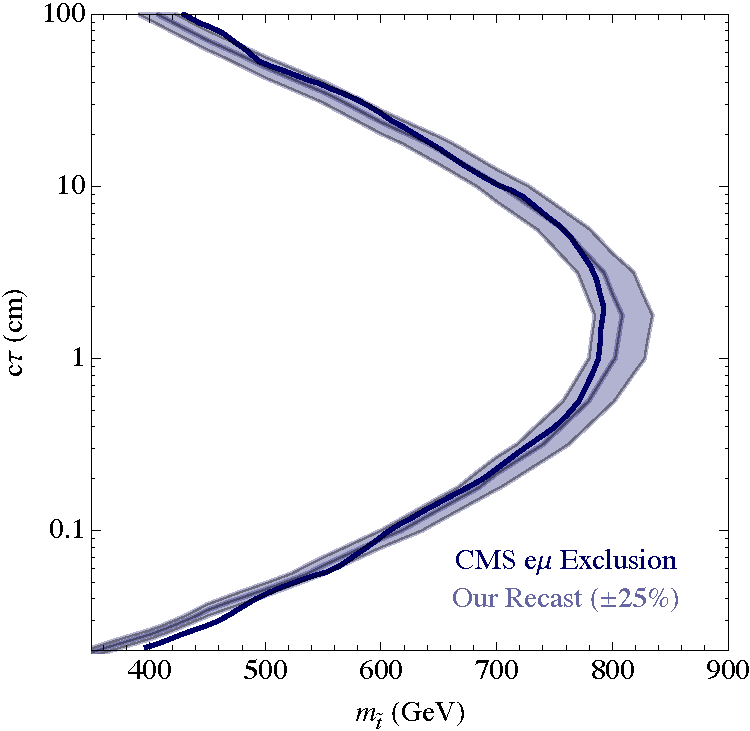
\includegraphics[width=0.65\textwidth,angle=0]{ch5-figures/emuVal.pdf}
\end{center}
\caption{Validation of the CMS displaced $e\mu$ search~\cite{Khachatryan:2014mea} for
  the displaced supersymmetry benchmark model
  \cite{Graham:2012th}.  Figure taken from \cite{Evans:2016zau}.
}
\label{fig:DTval}
\end{figure}

In Figure~\ref{fig:DTval}, we present the validation of the CMS displaced $e\mu$
search~\cite{Khachatryan:2014mea} from the study performed
in Ref.~\cite{Evans:2016zau}.  For this search, we show the recommended 25\% modeling
uncertainty~\footnote{A similar validation was done in Ref.~\cite{Liu:2015bma} with details
provided in its Appendix D. After applying a flat $80\%$ efficiency, a $20\%$ modeling uncertainty
is found to be appropriate, as shown in Fig.~14 of the reference}. The recast agrees
very well with the results from the CMS displaced
$e\mu$ search  in the region of highest sensitivity, 300 $\mu$m $\lesssim c\tau
\lesssim 50$ cm, but exhibits a moderate deviation on the tails.   As this
extremely low efficiency region is overly sensitive to the tails of kinematic
distributions, it may be the case that the sensitivity is slightly under-estimated
for lifetimes near 1 m or 100 $\mu$m, but this discrepancy typically has no
qualitative impact on any application of the results.

\subsubsection{Extrapolation to 13 TeV}

We now show another reinterpretation example of the CMS displaced $e\mu$ in
order to highlight the comparison between 8 TeV~\cite{Khachatryan:2014mea} and 
13 TeV~\cite{CMS-PAS-EXO-16-022} analyses. We compare in
Fig.~\ref{fig:ch5-valid1} our reproduction of expected signal events with the
published validation material for the 8 TeV version, and the partially-available
validation material for the 13 TeV search.
Information on efficiency maps from the 8 TeV analysis was needed
to obtain an extrapolation to 13 TeV, as the 13 TeV efficiency
 maps are not yet public.
As we can see, the 8 TeV recast for the CMS displaced lepton
search~\cite{Khachatryan:2014mea} agrees very well in the region of highest
sensitivity. The 13 TeV recasting, however, under-estimates the CMS values
by a factor of two or more. This is likely due to the fact that the
lepton efficiencies can not be directly extrapolated from 8 to 13 TeV,
as assumed in making Figure~\ref{fig:ch5-valid1}.
Also, with the absence of a cut-flow table, it is impossible to verify where the
mis-match arises, whether it is due to mis-modeling of the signal region
cuts or  due to genuine changes in the efficiencies.



\begin{figure}[ht]
\centering
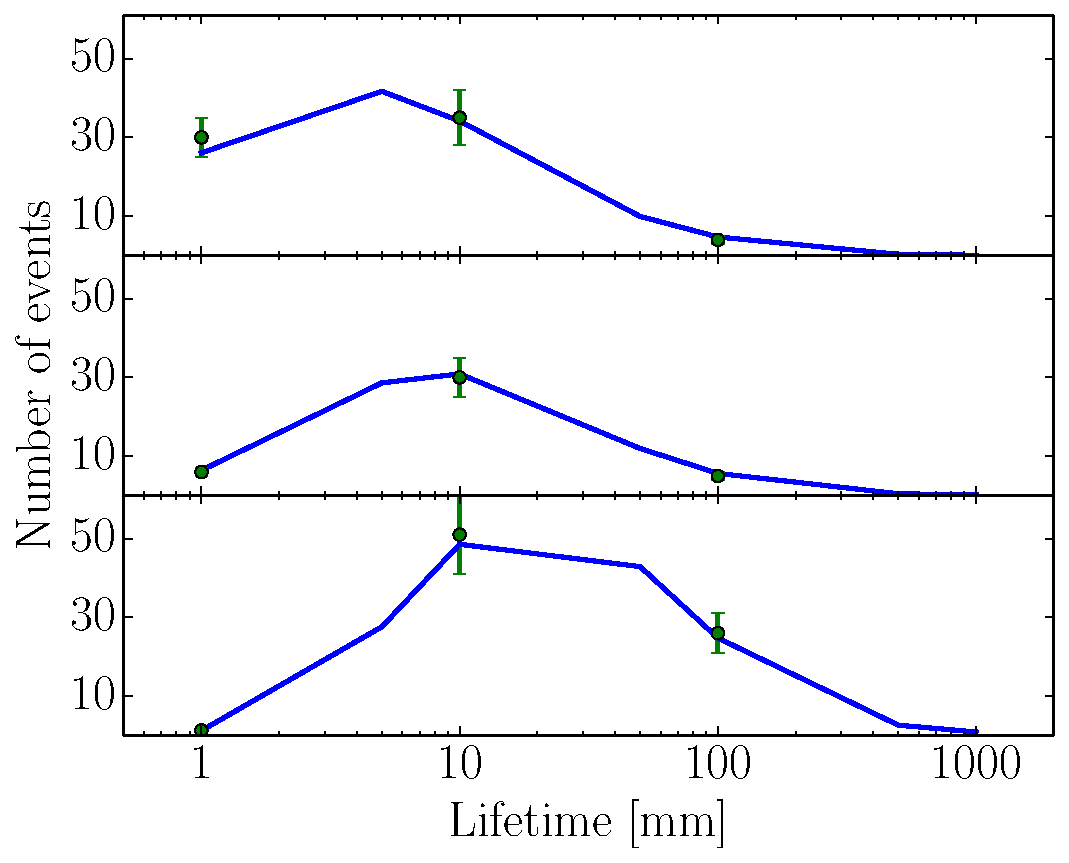
\includegraphics[width=0.48\textwidth,angle=0]{ch5-figures/disp_lep_8tev.pdf}
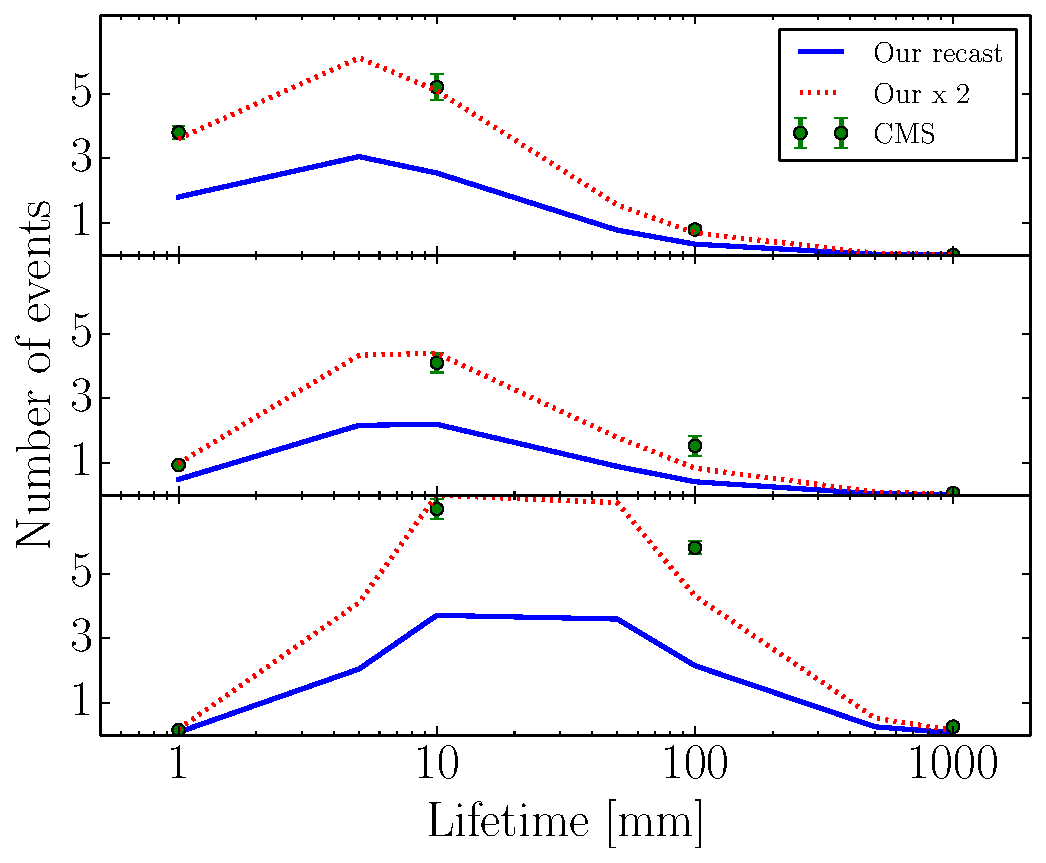
\includegraphics[width=0.48\textwidth,angle=0]{ch5-figures/disp_lep_13tev.pdf}


\caption{\label{fig:ch5-valid1} Number of expected events in the signal regions defined based on $|d_0|$ for the CMS displaced $e\mu$ search.  The green points refer to the expected signal published by the analysis. {\bf Left:} Validation for 8 TeV analysis.  Production cross section assumed NLO+NLL value 85.6 fb for $M_{\tilde t_1} = 500$ GeV, BR = 0.33 in each $\ell$-channel. {\bf Right:} Validation for 13 TeV analysis. Production cross section assumed NLO+NLL value 67.0 fb for $M_{\tilde t_1} = 700$ GeV. The 13 TeV numbers are made using efficiency maps published for the 8 TeV search, as the 13 TeV maps are not yet public. Figures taken from Ref.~\cite{LesHouches2017}.}
\end{figure}

\vskip 0.1in
\noindent {\bf Lessons learned}
\vskip 0.1in

The selection and trigger efficiencies provided by CMS
are very useful for recasting the 8 TeV CMS search for
displaced leptons~\cite{Khachatryan:2014mea}
and allow for a very good level of agreement.
The main challenge, however, consisted in collecting all the available
information, which was not provided by the main document in
Ref.~\cite{Khachatryan:2014mea}.
Furthermore, the corresponding information for the 13 TeV search is
not publicly available and an extrapolation of the 8 TeV efficiencies
was shown to be inadequate.

\subsection{Displaced Jets}
\label{displacedJets}

Searches for displaced jets are less straightforward to reinterpret than
displaced leptons. Interest in accurate reinterpretation is increasing, as many
new physics models give rise to this particular signature. The CMS search for
displaced di-jets~\cite{CMS-PAS-EXO-12-038} was reinterpreted in Ref.~\cite{Cui:2014twa} to explore
long-lived particle signatures for certain weak-scale models of
baryogenesis~\cite{Cui:2012jh,Cui:2013bta,Cui:2014twa}, as well as a study~\cite{Liu:2015bma} to
understand current limits on long-lived signatures in supersymmetry.

The CMS search~\cite{Cui:2014twa}  uses a multivariate discriminant 
composed of observables that are
challenging to model in Monte Carlo, such as the  track-multiplicity of the vertex
and the root-mean-square of a cluster track-multiplicity variable. The
reinterpretation approach in Refs.~\cite{Cui:2014twa,Liu:2015bma} was to construct track
information at truth level based on the output of a parton shower program (such
as {\sc{Pythia 8}}), and then use the truth-level information to construct the
various vertex, cluster, and track-level observables for each event. As it is
difficult to adequately account for inefficiencies of track and vertex
reconstruction, the efficiency of passing the cuts with truth-level observables
was considered and then it was normalized to the results from CMS. To do so, the
authors of Ref.~\cite{Cui:2014twa}
simulated identical signal models to those with efficiencies reported by the CMS
collaboration, assumed that the MC truth-level reconstruction gave an adequate
description of kinematics but \emph{not} track and vertex reconstruction, and so
computed a ratio of truth-level efficiencies to those reported by CMS. The resulting
 efficiency ratios were used to re-scale the truth-level results of other models,
leading to a reinterpretation of the CMS search for different models beyond the
ones they considered. The details can be found in Ref.~\cite{Cui:2014twa};
 a more sophisticated approach in which object efficiencies were estimated and applied
  to tracks and displaced vertices  in Ref.~\cite{Liu:2015bma}.

To validate this approach, truth-level quantities for the models constrained in
Ref.~\cite{CMS-PAS-EXO-12-038} were computed and compared to the numbers and
distributions reported. For example,
comparisons of the distributions of the observables going into the multivariatereinterpretation
discriminant, as well as the output of the multivariate discriminant could be
performed. While the truth-level distributions disagreed with those of CMS for
individual observables, the actual multivariate discriminant output agreed with
that of CMS at better than 25\%. The ratio of truth-level efficiencies to CMS
efficiencies are also compared for different LLP masses and kinematics, and
these typically agree with one another at the factor-of-two
level~\cite{Cui:2014twa}. This suggests that this reinterpretation of the CMS
results in terms of cross-section limits is likely accurate to the factor-of-two level.

\vskip 0.1in
\noindent {\bf Lessons learned}
\vskip 0.1in

We find that a rather na\"ive truth-level reconstruction of the event could give a reinterpretation of cross-section limits to agree within a factor of two, provided the efficiencies were normalized to the experimental values using an overlapping set of signal models. One of the major obstructions to improving  the accuracy of the estimate was the model dependence observed among the ratios of efficiencies between truth-level information and CMS. For instance, it was found that highly boosted models showed a much lower relative reconstruction rate in data vs.~truth-level MC than less-boosted LLPs. Since pair production of LLPs was considered near threshold in Ref.~\cite{Cui:2014twa}, this degradation in the performance of highly boosted LLPs does not greatly affect the confidence in the final result. However, it does suggest that characterizing the effects of the particle boost are important for reinterpretation.

In addition, with a larger and more diverse set of signal benchmarks available, the prospects for the reinterpretation of search results are better. The reasons are twofold:~
%
\begin{itemize}
\item Increasing the number of presented signal models by the collaboration allows for more cross-checks between MC and the results in data. This allows for more sophisticated tuning of efficiencies as applied to truth-level events;
\item Having a more diverse set of benchmark signal models means that it is easier to disentangle various kinematic effects on the efficiency (such as the LLP mass, boost, etc.) and find a signal benchmark that most closely matches the model for which one wants to derive sensitivity.
\end{itemize}
%

\subsection{Displaced Lepton Jets}

A variety of scenarios predict the existence of LLPs decaying to a pair of highly collimated leptons, also known as lepton jets (LJs) \cite{ArkaniHamed:2008qp}. Models giving rise to LJ signatures include heavy right-handed neutrinos, exotic Higgs decays, and dark gauge bosons. The relevant signature is one or more LJs emerging from a DV. In many cases, there can also be associated prompt objects, such as a prompt lepton produced in conjunction with the right-handed neutrino (corresponding to charged-current production in the simplified model framework of Sec.~\ref{sec:proposal}.

\paragraph {Existing searches} Current search results are outlined in Section~\ref{subsec:dleptons}. The search in Ref.~\cite{ATLAS:2016jza} was interpreted in the framework of the Falkowski-Ruderman-Volanksy-Zupan (FRVZ) model~\cite{Falkowski:2010cm} for the Higgs boson interacting with a hidden sector containing a massive dark photon ($\gamma_d$), massive neutralinos, and three hidden scalars. Displaced LJs are produced at the end of Higgs cascade decay that also yields two hidden light stable particles (HLSPs). Depending on the hidden-sector spectrum, the cascade decay may yield two or more $\gamma_d$ that each decay to pairs of Standard Model charged particles via kinetic mixing with the hypercharge gauge boson. The $\gamma_d$ decay products are highly collimated. For $m_{\gamma_d} < 500$ MeV, LJs are the dominant decay mode, while for larger dark photon masses, displaced hadronic jets can also be significant.

Results are presented as limits on $\sigma\times \mathrm{BR}(H\to n\gamma_d+X)$ ($n=2$, 4) as a function of the $\gamma_d$ $c\tau$. The strongest limits  from the 8 TeV dataset are events require at least one LJ with muons. For $n=2$, a $\sigma\times \mathrm{BR}(H\to 2\gamma_d+X)$ of $\gtrsim1$ pb is excluded for $c\tau\sim 50$ mm.

\paragraph {Recast: Dark Photon with Non-Abelian Kinetic Mixing} The FRVZ model on which the ATLAS analysis was based implies the presence of at least two displaced LJs in the final state as well as two additional unobserved HLSP's that corresponding to missing energy. The ATLAS analysis did not impose any \MET cuts. The presence of the two HLSPs affects the kinematics and topology of the signal event but does not explicitly enter the event selection or reconstruction. Thus, one should be able to reinterpret the ATLAS analysis in terms of any other model containing two or more displaced LJ, along with potentially additional, unobserved objects.

%Models containing heavy right-handed neutrinos can yield events with one DV LJ, \MET and a prompt lepton -- a topology that is not easily matched to the ATLAS DV LJ analysis. Alternatively, 
We consider a scenario for a dark photon $X_\mu$ that mixes with the neutral Standard Model SU(2$)_L$ gauge boson $W_\mu^3$ via a higher dimensional operator. Two possibilities have recently been considered: a dimension six operator involving the SM Higgs doublet, the SU(2$)_L$ field strength $W_{\mu\nu}^a$ and the corresponding U(1$)^\prime$ field strength $X_{\mu\nu}$~\cite{Barello:2015bhq}; and a dimension five operator involving $W_{\mu\nu}^a$, $X_{\mu\nu}$, and a real scalar triplet $\Sigma\sim (1,3,0)$~\cite{Arguelles:2016ney}. We consider the latter since it can yield an event topology similar to that of the FRVZ model and since it is the leading operator that may generate non-abelian kinetic mixing (NAKM) of the U(1$)^\prime$ gauge boson with the SM. We will henceforth refer to this model as the NAKM5 scenario.
%
The corresponding operator is
\begin{equation}
\label{eq:ch5-dimensionfive}
\mathcal{O}_{WX}^{(5)} =
-\frac{\beta}{\Lambda}\,\text{Tr}\left(W_{\mu\nu}\Sigma\right) X^{\mu\nu}
\end{equation}
where $\Lambda$ is the associated effective field theory mass scale and $\beta$ is a dimensionless coupling that is nominally $\mathcal{O}(1)$. When the neutral component of the $\Sigma$ obtains a vacuum expectation value (vev) $v_\Sigma$, one has the ratio of the dark photon and SM photon couplings
\begin{equation}
\label{eq:ch5-dimfiveeps}
\epsilon = {\beta\sin\theta_W}\, \left(\frac{v_\Sigma}{\Lambda}\right)\ \ \  .
\end{equation}
Note that the $\rho$-parameter constrains $v_\Sigma$ to be smaller than about \mbox{4~GeV}. Consequently, for $\Lambda$ of order one TeV, $\epsilon$ is small (and consistent with present experimental constraints) without requiring the presence of a suppressed coupling in the Lagrangian. This feature distinguishes the dimension-five non-abelian kinetic mixing from the dimension four kinetic mixing between $X_\mu$ and the SM hyper charge gauge boson.

The final state with two $\gamma_d$ (resulting from the $X_\mu$-$W_\mu^3$ mixing) can be produced in one of two ways: (a) electroweak Drell-Yan pair production of  triplet scalars that subsequently decay to a $\gamma_d$ and SM gauge boson via the operator in Eq.~\eqref{eq:ch5-dimensionfive}; (b) production of the $\gamma_d$ and a triplet scalar via $\mathcal{O}_{WX}^{(5)}$ with a subsequent decay of the triplet to a second $\gamma_d$ plus a SM gauge boson via the same operator. In each case, one would expect the presence of two $\gamma_d$ plus one or more unobserved massive prompt bosons in the final state. The ATLAS DV plus LJ analysis can be recast in a straightforward way for these event topologies, as no information about the unobserved prompt object has been used. It is worth emphasizing that both the production processes as well as the $\Sigma$ decay rate are independent of the triplet vev, $v_\Sigma$. The latter only enters $\epsilon$ and, thus, only affects the dark photon $c\tau$.

\begin{figure}[!t]\centering
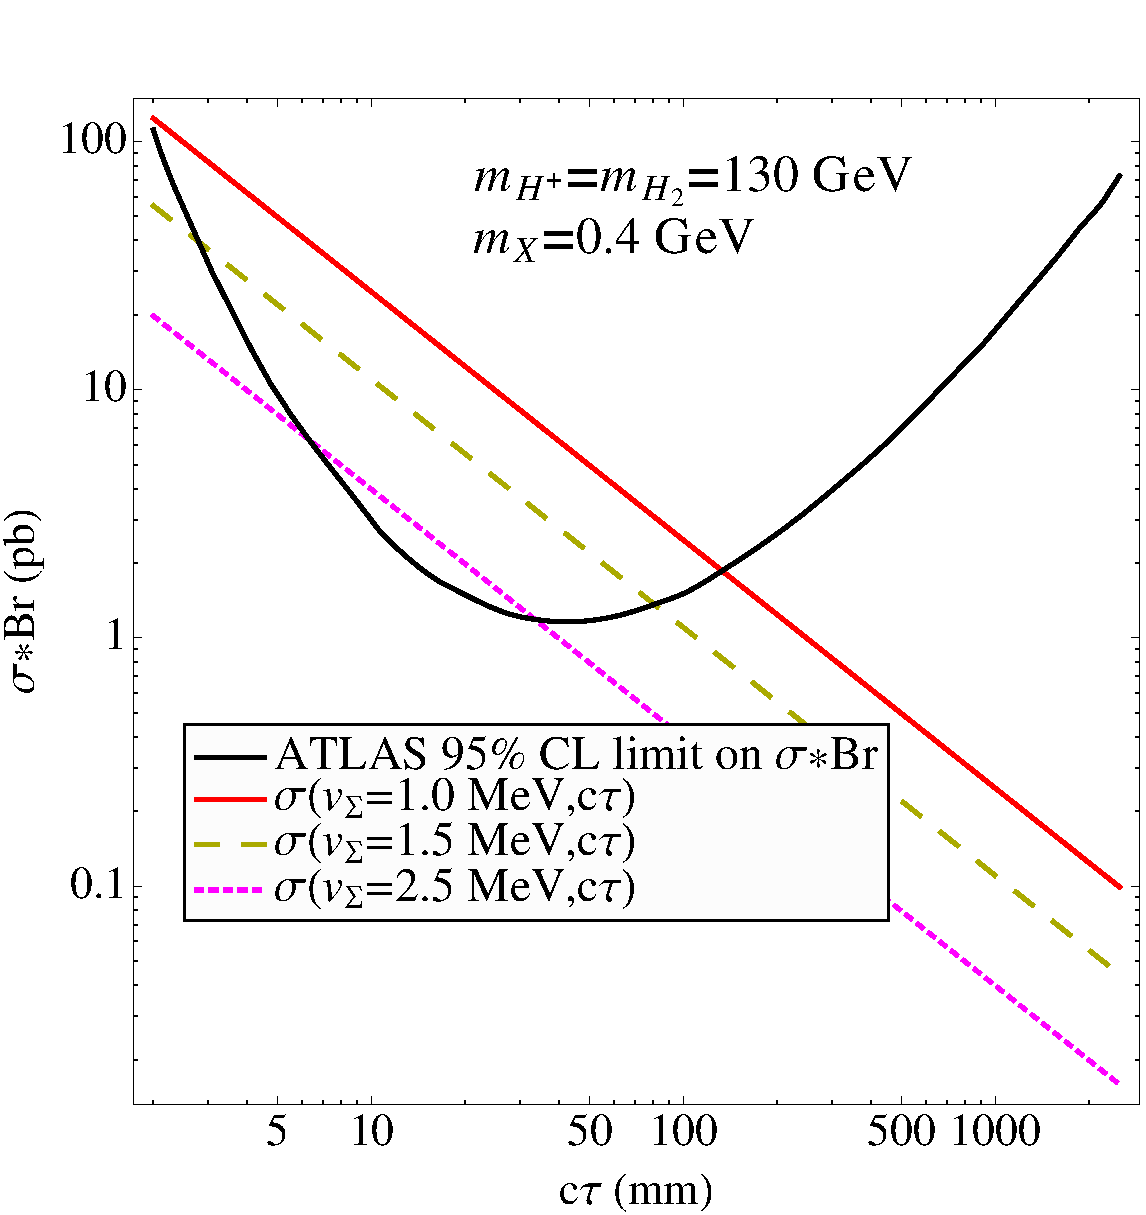
\includegraphics[width=0.48\textwidth,angle=0]{ch5-figures/dvlj_atlas_recast_0.pdf}\hspace*{2mm}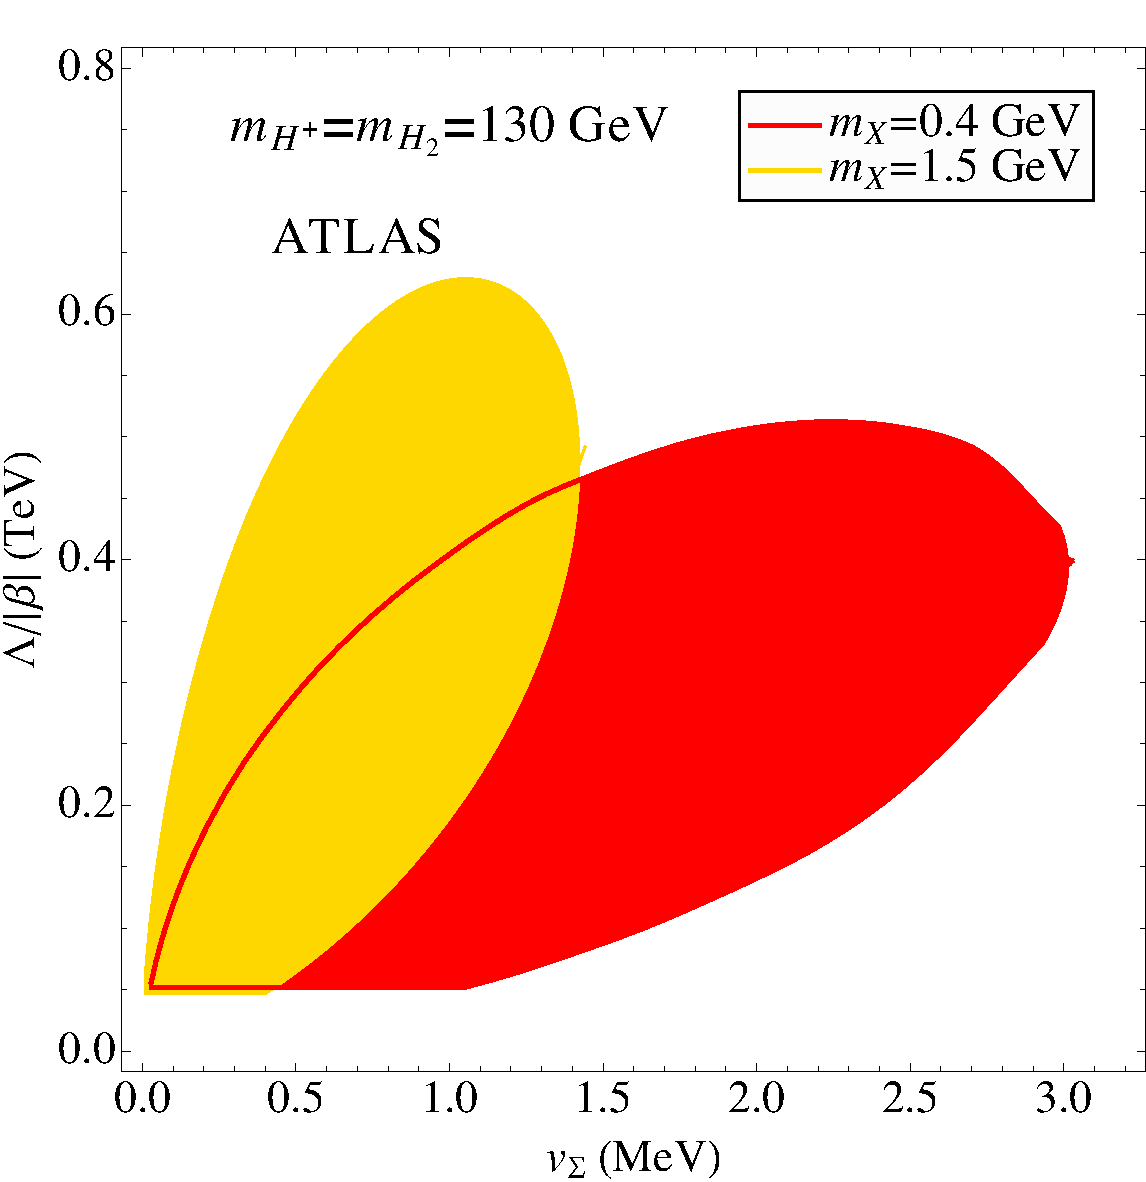
\includegraphics[width=0.48\textwidth,angle=0]{ch5-figures/dvlj_atlas_recast.pdf}
\caption{Constrains on the NAKM5 scenario, recast from the ATLAS search reported Ref.~\cite{Aad:2014yea}. The left panel gives the exclusion in the ($c\tau$, $\sigma\times\text{BR}$) plane, where the region above the parabola is excluded. The diagonal lines indicate the dependence of $\sigma\times\text{BR}$ on $c\tau$ for different representative choices of $v_\Sigma$. The right panel gives the exclusion region in the($v_\Sigma$, $\Lambda/\beta$) plane for $m_X=0.4$ GeV (red region) and $m_X=1.5$ GeV (yellow region).} % {\color{magenta} need PLB reprint permission statement}}
\label{fig:ch5-ATLASbounds}
\end{figure}

The corresponding implications of the ATLAS 8 TeV results are indicated in Fig.~\ref{fig:ch5-ATLASbounds}. The first panel shows the limits on the $\sigma\times\mathrm{Br}$ as a function of $c\tau$. The corresponding model sensitivity is shown for different choices of $v_\Sigma$ by the diagonal lines. Note that for fixed $v_\Sigma$ both the $\sigma\times\mathrm{Br}$ and $c\tau$ depend on the operator coefficient $\beta/\Lambda$, leading to a non-trivial relationship between the two experimental quantities. This situation differs from the FRVZ model, where $\sigma\times\mathrm{Br}$ is independent of $c\tau$ since the mixing parameter $\epsilon$ does not depend on the parameters governing production of the hidden sector particles or their cascade decays. The intersections of the model lines with the ATLAS limits can then be translated into bounds on $\Lambda/\beta$ as a function of $v_\Sigma$ for different choices of the dark photon mass (denoted here as $m_X$), as shown in the second panel of Fig.~\ref{fig:ch5-ATLASbounds}. For a 1.5~GeV dark photon, the excluded region reaches \mbox{600~GeV} for $v_\Sigma = 1 $ MeV.

The aforementioned recast does not require detailed information on event topology, other than the dark photon decay length. Consequently, the 13~TeV limits  \cite{ATLAS:2016jza} translate rather straightforwardly into stronger bounds on the model parameter space, reaching to somewhat larger $\Lambda/\beta$.

\vskip 0.1in
\noindent {\bf Lessons learned}
\vskip 0.1in

The triggering requirements used in the ATLAS analysis thus far limit the reach of displaced LJ searches. For models having a signal with only the displaced LJ and no other observable objects, such as the FRVZ model, triggering solely on MS tracks not associated with ID tracks is appropriate, though even here the 3mu6 trigger may not be sufficiently inclusive, as it requires at least three ROIs in the MS (see Sec.~\ref{sec:CMSleptonic}). Events with LJ pairs for which neither LJ can be resolved into two separate ROIs will be missed.

It is clear that triggering on associated prompt objects, such as the lepton from one of the final state vector bosons in the NAKM5 scenario or from the $W$ boson in heavy right-handed neutrino models (charged-current LLP production), could significantly enhance the triggering efficiency and extend the reach of displaced LJ searches to a wider class of models and to a broader range of model parameter space. Inclusion of an associated prompt object in triggering may also enhance background rejection and relax the requirement on $\Delta\phi$ between LJs.

In addition, the implications of the mass scale of the intermediate BSM particles and the number of finial state prompt objects remains to be investigated. The ATLAS 8 TeV search assumed the hidden sector particles are light compared to the mass of the SM Higgs boson, whose decay chain leads to the final states involving multiple $\gamma_d$ and HLSPs. For the NAKM5 scenario and models with heavy right-handed neutrinos, these assumptions about mass hierarchy may not apply. It is also not clear what impact the DV LJ isolation requirements have when there is an associated prompt lepton in the signal event.



\subsection{Non-pointing Photons}

The search for non-pointing photons produced in association with missing
transverse energy ($\slashed E_T$)~\cite{Aad:2014gfa} plays an important role in probing beyond-the-SM (BSM) particles that decay to a SM photon and an invisible particle through a highly suppressed coupling. Beside the gauge-mediated supersymmetry breaking (GMSB) models~\cite{Dine:1981gu}, which were the main motivation for the non-pointing photon search, this type of signal can also appear in many hidden-sector models. For example, in the dipole-mediated DM model (the ``Dark Penguin'')~\cite{Primulando:2015lfa}, the production of two heavier dark fermions $pp\to Z^*/\gamma^*\to\chi_h\bar{\chi}_h$ is followed by the decays $\chi_h \to \chi_l+ \gamma$. If the flavor structures of the DM mass and coupling are aligned, $\chi_h$ can be long-lived and give rise to non-pointing photons. Another example is provided by the dark-shower scenario~\cite{Freytsis:2014sua,Freytsis:2016dgf} that explains the galactic center gamma-ray excess. In this model, many hidden pions can be produced in the same LHC event. Some of these have displaced decays to a pair of SM photons, while others decay outside of the detector, yielding $\slashed E_T$. Notice that in this case the topology of the events is different from the previous examples, as the non-pointing photons and $\slashed E_T$ originate from separate particles (for more discussion on dark showers, see Chapter~\ref{sec:showers}).

Here, we describe a method used to recast the bounds of
Ref.~\cite{Aad:2014gfa} to a BSM scenario that is different from the GMSB model,
using the Dark Penguin signal \cite{Primulando:2015lfa} as an example.

\begin{figure}[t]
\begin{center}
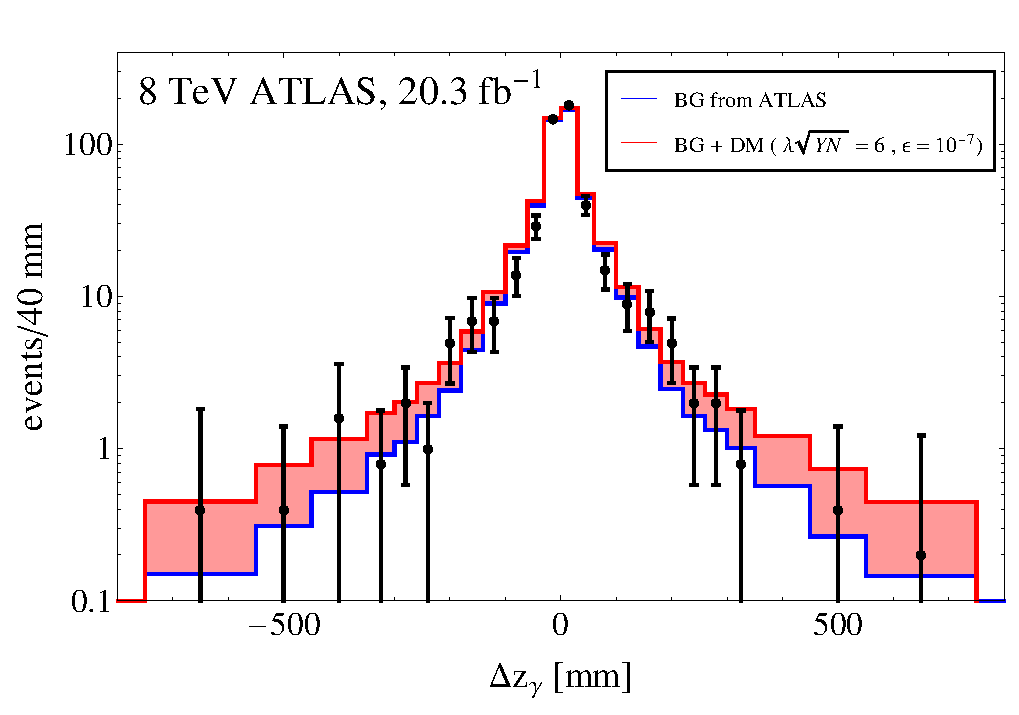
\includegraphics[width=0.45\textwidth]{ch5-figures/nonpointing_photon}\qquad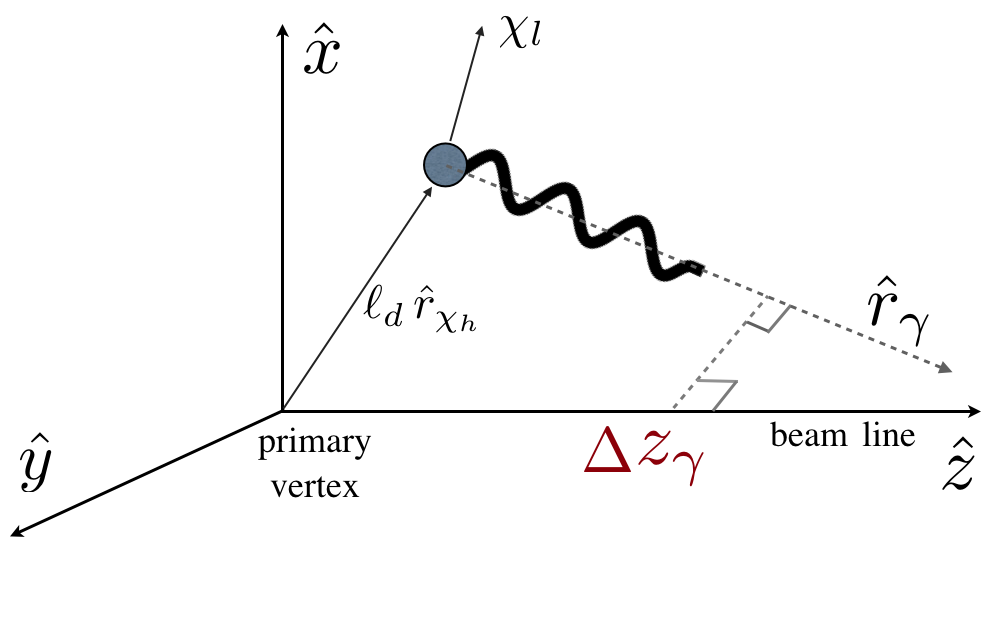
\includegraphics[width=0.45\textwidth]{ch5-figures/displaced_cartoon}
\end{center}
\caption{{\bf {Left}}: the $\Delta z_{\gamma}$ distribution of the non-pointing photon signals measured by ATLAS. The background reported by ATLAS (blue histogram) was obtained from a data-driven analysis, using diphoton events with $\slashed E_T<20$ GeV. Also shown, stacked on top of the background (red histogram), is the signal distribution from the dipole-mediated DM scenario with $(m_{\chi_h},\,m_{\chi_l},\,M)=(300,\,10,\,300)$ GeV, $\lambda\sqrt{NY}=6$, and $\varepsilon=10^{-7}$. See Ref.~\cite{Primulando:2015lfa} for more details. {\bf{Right}}: the geometry of the displaced signals.}
\label{fig:nonpointing}
\end{figure}

%%%%%%%%
\subsubsection{Calculation of the signal efficiency for the non-pointing photon search}
%
We follow the non-pointing photon analysis in Ref.~\cite{Aad:2014gfa}, performed
by the ATLAS collaboration on about $20$ fb$^{-1}$ of $8$ TeV data. In
Ref.~\cite{Aad:2014gfa} delayed photons were also considered, but here we focus
only on the measurement of the $\Delta z_{\gamma}$ of non-pointing photons (see
Fig.~\ref{fig:nonpointing}). For DM signals given by the long-lived
$\chi_h\to\chi_l\gamma$ decay, $\Delta z_{\gamma}$ can be related to the
$\chi_h$ decay length $\ell_{d}$ in the lab frame:
\begin{eqnarray}\label{eq:Zgamma}
\Delta z_{\gamma}&=&\ell_d\left(\hat{r}_{\chi_h,z}-\frac{\hat{r}_{\chi_h,T}\cdot\hat{r}_{\gamma,T}}{1-(\hat{r}_{\gamma,z})^2}\hat{r}_{\gamma,z}\right)\nonumber\\
& =& \ell_d \Big[\cos\theta_{\chi_h} -\cos (\phi_{\chi_h} - \phi_\gamma)\mathrm{cot}\,\theta_\gamma \sin \theta_{\chi_h} \Big]
\end{eqnarray}
where $\hat{r}_{T,z}$ represent the transverse and longitudinal components of
the unit vector $\hat{r}$, respectively, as shown in
the right pane of Fig.~\ref{fig:nonpointing}.
To obtain the $\Delta z_{\gamma}$ distribution of the DM decay, we first
simulate the prompt process, $p\,p \to \chi_h\bar{\chi}_h,
\chi_h\to\chi_l\gamma, \bar{\chi}_h\to\bar{\chi}_l\gamma$ in MadGraph5, then we
apply the cuts performed in the ATLAS analysis, and finally reweight the events
using the dark penguin form factors. Then we calculate the proper lifetime of
$\chi_h$ and boost it to the lab frame using the momenta of each parton-level
event. The angular information of the photon and $\chi_h$ allow us to calculate
$\Delta z_{\gamma}$ in Eq.~\eqref{eq:Zgamma} as a function of the decay length.
Using this, each simulated MC event contributes to the differential cross
section in $\Delta z_{\gamma}$ as
\begin{equation} \label{eq:displdistr}
\frac{d\sigma_{\text{displaced}}}{d\Delta z_{\gamma}} =\sigma_{\text{prompt}}\frac{d\,P}{d\Delta z_{\gamma}}=\sigma_{\text{prompt}}\frac{|\mu|}{2} e^{-\mu\,\Delta z_{\gamma}},
\end{equation}
where the $\mu$ characterizing the probability distribution $dP/d\Delta z_\gamma$ of the decay is defined as
\begin{equation}
\mu\equiv\frac{\Gamma_{\chi_h}m_{\chi_h}}{p_{\chi_h}}\left(\hat{r}_{\chi_h,z}-\frac{\hat{r}_{\chi_h,T}\cdot\hat{r}_{\gamma,T}}{1-(\hat{r}_{\gamma,z})^2}\hat{r}_{\gamma,z}\right)^{-1}.
\end{equation}
Summing the distributions derived from all the simulated events we obtain the
differential cross section in $\Delta z_\gamma$ shown in Fig.~\ref{fig:nonpointing}.

The ATLAS search requires at least two loose photons with $|\eta|<2.37$ and $E_T>50$ GeV. At least one photon is required to be in the barrel region $|\eta|<1.37$. To avoid collisions due to satellite bunches, both photons are required to have an arrival time at the ECAL $t_{\gamma}$ smaller than $4$ ns, with zero defined as the expected time of arrival for a prompt photon from the primary vertex. We approximate $t_\gamma$ with the time of flight of the $\chi_h$, requiring it to be smaller than $4$ ns.
In our sensitivity estimate, we do not include the detailed isolation cuts on the photon. We also neglect the effect of the displaced decay on the angular acceptance of the photons, simply imposing the requirements on $|\eta|$ at the level of the prompt event.
The signal region also requires $\slashed E_T>75$ GeV.
Finally, to simplify the discussion we assume that every event has a
reconstructed primary vertex in the geometrical center of the detector.


For events where only one photon satisfies $|\eta|<1.37$ (i.e. it is in the
barrel calorimeter), this photon is used for the measurement of $\Delta
z_{\gamma}$. For events where both photons are in the barrel, the photon with
larger $t_{\gamma}$ is used. We approximate this timing condition by taking the
photon emitted by the more boosted $\chi_h$, in which case the average decay is
more delayed. In Fig.~\ref{fig:nonpointing} the generated $\Delta z_{\gamma}$ signal distribution is shown on top of the expected background. The latter is taken from Fig.~4 of the ATLAS paper \cite{Aad:2014gfa}. Because we are focusing on the non-pointing photon signals, to set constraints on the DM couplings in Ref.\cite{Primulando:2015lfa} we remove events with $|\Delta z_{\gamma}|< 30$ mm. In our exploratory analysis we only consider the statistical uncertainty on the background, neglecting the effect of systematics.

\vskip 0.1in
\noindent {\bf Lessons learned}
\vskip 0.1in

The ATLAS paper gives detailed descriptions of the cuts and background analysis, which makes an approximate estimation of the signal efficiency quite straightforward.

The background analysis in Ref.~\cite{Aad:2014gfa} is based on a data-driven study, for which events passing the diphoton selection with $\slashed E_T<20$ GeV are used as control region sample. It is challenging for theorists to simulate the background for different energy cuts. This is particularly true for the $\slashed E_T$ cut that plays a vital role in the DM and Hidden Valley searches.

To obtain a more precise result, it would be useful if the ATLAS collaboration could provide the reconstruction efficiency of non-pointing photons as function of $\Delta z_{\gamma}$, or of the angle between the photon and the surface of the ECAL, a variable that may be relevant to the efficiency. The paper does provide a table of signal acceptance times efficiency for the GMSB SPS8 model. However, the numbers depend on details of the SPS8 model, and it is hard to extract the efficiency that is associated to the non-pointing photon reconstruction. Therefore, when estimating the signal efficiency, we only consider efficiency from the selection cuts and do not include possible suppressions from photon reconstruction.

It would also be very useful to have a table of background events for different cuts on $\slashed E_T$. For instance,  the Dark Penguin signature has $\slashed E_T$ from the decay of $\chi_h\bar{\chi}_h$ with electroweak-scale $m_{\chi_h}$, and \met can easily be higher than $100$ GeV. By contrast, in the dark shower scenario where soft hidden pions decay to two SM photons, the $\slashed E_T$ originating from additional late-decaying pions can be much lower than the $75$ GeV cut used in the ATLAS analysis. Knowing the background and systematic uncertainty for different $\slashed E_T$ cuts would be very important to constrain different models with potentially very different kinematics.


\subsection{Displaced Vertices}
\label{sec:ch5-displacedVertices}

Displaced-vertex searches differ from displaced jets and displaced leptons due to the requirement of an actual secondary vertex from the displaced objects. These searches are sensitive to LLP lifetimes that allow it to decay in the inner trackers or
muon spectrometer of the LHC detectors, where vertexing is possible~\cite{Aaboud:2017iio,Aad:2015rba,Aad:2015uaa,CMS:2014wda,CMS:2014hka,Aaij:2016xmb,Aaij:2017mic}. These searches have  extremely low background,s as there are no irreducible contributions from the SM, making them sensitive to very small signals of new physics (for more information, see Chapter \ref{sec:backgrounds}). Moreover, the identification of displaced decays can be used to extract kinematical information in a decay, such as (invisible) particle masses~\cite{Cottin:2018hyf,Park:2011vw}.

In this section we review some reinterpretations of displaced-vertex searches, differentiating between reinterpretations making use of only truth-level information to identify displaced decays and reinterpretations in which an attempt is made to reconstruct displaced vertices from displaced tracks (with an approximate detector response).

\subsubsection{Truth Level Displaced Vertices}

The work in Ref.~\cite{Cui:2014twa} reinterpreted the 8 TeV ATLAS search for a displaced muon and a multi-track vertex (DV+$\mu$)~\cite{ATLAS-CONF-2013-092}, where long-lived particle signatures for certain weak-scale models of baryogenesis~\cite{Cui:2012jh,Cui:2013bta,Cui:2014twa} were explored. For reinterpreting this search, a similar procedure described in the displaced jets
section~\ref{displacedJets} of constructing ratios of truth-level vs.~ATLAS efficiencies for the ATLAS multi-track vertex analysis~\cite{ATLAS-CONF-2013-092} was performed, with similar results for the validation being correct within approximately a factor of two.

This DV+$\mu$ analysis has since been superseded by Ref.~\cite{Aad:2015rba}, in which a displaced vertex is searched at 8 TeV in association with either a muon, electrons, jets and missing transverse momenta. Recently, an updated ATLAS analysis~\cite{Aaboud:2017iio}, which looks for multi-track displaced vertices at 13 TeV in association with large \met, was made public. This search now includes a prescription using parametrized efficiencies as a function of vertex radial distance, number of tracks and mass. Their prescription can be applied to vertices and events passing certain particle level acceptance requirements using the truth MC event record.

Here we validate the prescription with parametrized selection efficiencies
in Ref.~\cite{Aaboud:2017iio}~\footnote{This prescription is also validated in
Ref.~\cite{LesHouches2017}.}. The results of this search are interpreted by ATLAS in a split-SUSY simplified model with a long-lived gluino that hadronizes, forming an $R$-hadron before decaying as $\tilde{g}\rightarrow q\bar{q}\tilde{\chi}^{0}_{1}$. Event samples are generated with \textsc{Pythia 8.2}~\cite{Sjostrand:2014zea}. We use truth-level \met and we identify the truth $R$-hadron decay position and decay products, as the ATLAS collaboration provides selection efficiencies that can be directly applied to these truth-level quantities. These efficiencies can be found in the auxiliary material in Ref.~\cite{SUSY-2016-08}, and are given at the event-level as a function of the truth \met and displaced-vertex radial distance, and at the vertex level parametrized as function of vertex invariant mass and number of tracks. The efficiencies are given for different detector regions, encapsulating also the effect of the material veto cut.

The selection of events used for the signal region requires:
%
\begin{itemize}
\item{truth level $\metm>200$ GeV;}
\item{one trackless jet with $p_{T}>70$ GeV, or two trackless jets with $p_{T}>25$ GeV. A trackless jet is defined as a jet with $\sum_{tracks} p_{T}<5$ GeV.}
\end{itemize}

In addition, events must have at least one displaced vertex with:

\begin{itemize}
\item{transverse distance between the IP and the decay position $>4$ mm;}
\item{the decay position must lie in the fiducial region $r_{DV}<300$ mm and $|z_{DV}|<300$ mm;}
\item{the number of selected decay products must be at least 5, where selected decay products are charged and stable, with $p_{T}>1$ GeV and $|d_{0}|>2$ mm;}
\item{the invariant mass of the truth vertex must be larger than 10 GeV, and is constructed assuming all decay products have the mass of the pion.}
\end{itemize}

Applying these cuts and efficiencies, we get event-level efficiencies for two of
the benchmarks (with gluino masses of 1400 GeV or 2000 TeV, and the
neutralino mass is fixed to 100 GeV). Based on the efficiencies obtained and the
estimated number of background vertices, we can extract 95\% CL upper limits on
the total visible cross section for the two gluino masses. For reference,
assuming $100\%$ efficiency, we get an upper limit of $0.091$ fb. The
curves in Figure~\ref{fig:DVsigmaLimits} show our recasting results compared to
ATLAS. The level of agreement is very good, within 20\% for most of the
lifetime values. We also point out that the recasting limits agree well
even for regions where the efficiency is very low ($\tau > 10$~ns
and $\tau < 10^{-2}$~ns).
This 13 TeV ATLAS multitrack analysis~\cite{Aaboud:2017iio} has also been reinterpreted in the
context of long-lived sterile neutrinos~\cite{Cottin:2018nms,Cottin:2018kmq}.

\begin{figure}[t]
\begin{center}
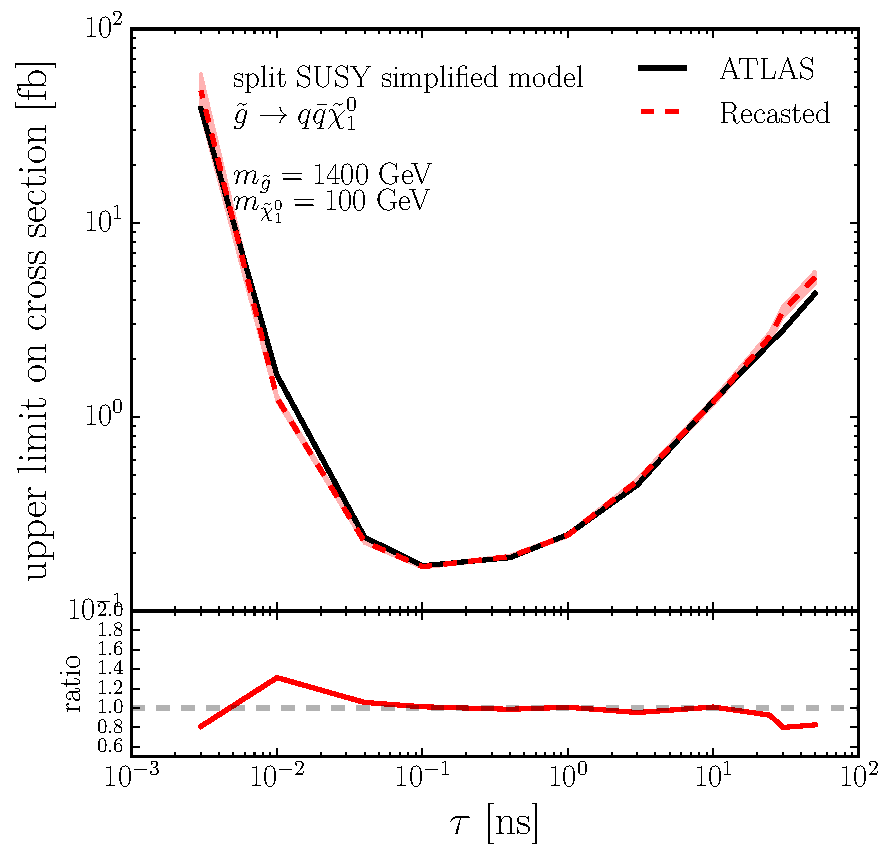
\includegraphics[width=0.45\textwidth]{ch5-figures/limits_gluino1_FIXED.pdf}
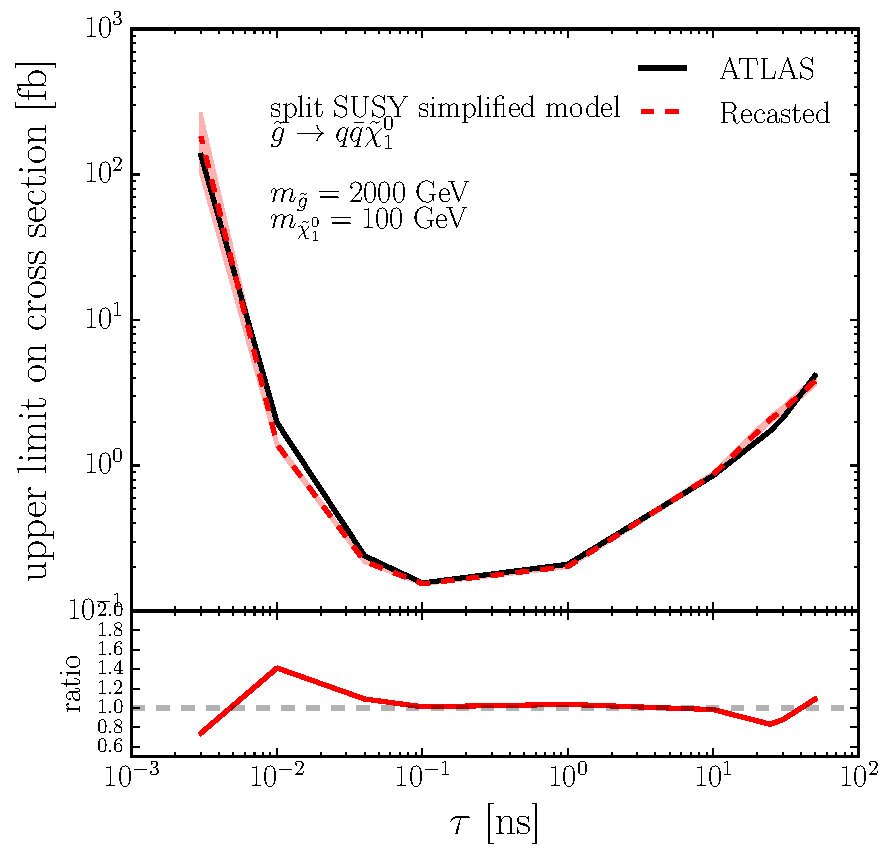
\includegraphics[width=0.45\textwidth]{ch5-figures/limits_gluino2_FIXED.pdf}
\caption{ Comparison of our recast and ATLAS~\cite{Aaboud:2017iio} on the upper limit in the gluino production cross section against its proper lifetime~\cite{LesHouches2017}.}
\label{fig:DVsigmaLimits}
\end{center}
\end{figure}

\subsubsection{Displaced-Vertex Reconstruction}
\label{sec:ch5-displacedVertexReconstruction}
Before parametrized efficiencies applicable for truth-level displaced vertices were made public, attempts to recast displaced-vertex searches were made by performing their reconstruction from charged tracks only, with an approximate detector response. In Ref.~\cite{Allanach:2016pam} the ATLAS DV+jets multitrack analysis~\cite{Aad:2015rba} was recast. Reinterpretation was performed using generator-level events and the detector fiducial region was reproduced as well as possible.  The jets are clustered according to the anti-$k_T$ prescription \cite{Cacciari:2008gp} in the analysis with momentum smearing (this is validated by reproducing the jets+\MET exclusion curve of prompt searches).  The selection of events used for the signal region (and the approximations to real detector simulation) were as follows:
%
\begin{table}[ht]
\footnotesize
\begin{center}
% \begin{tabular}{|p{3.0cm}p{12.5cm}|}
\begin{tabular}{|p{2.0cm}p{7cm}|}
\hline
{ DV jets}     & 4 or 5 or 6 jets with  $|\eta| <2.8$ and $p_{T} > 90, 65,
55$ GeV, each\\
 & \\
{ DV reconstruction}$^*$   & DV made from tracks with $p_{T}>1$ GeV, $|\eta|<2.5$ and $|d_{0}|>2$ mm. Vertices within 1 mm are merged. Note: a tracking efficiency needed here; we assume a functional form given by equation~\ref{eqn:trkeff} \\
 & \\
{  DV fiducial}         & DV within $4$ mm $<r_{DV}<300$ mm and $|z_{DV}|<300$ mm
\\
 & \\
{ DV material}$^*$         & No DV in regions near beampipe or within pixel layers. Discard tracks with

$r_{DV}/\mathrm{mm} \in \{[25,38], [45,60], [85,95], [120,130]\}$.\\
                    & \\
                    & \\
 $N_{\rm trk}$       & DV track multiplicity $\geq 5$ \\
 & \\
  $m_{DV} $         & DV mass $>10$ GeV \\
\hline
\end{tabular}
\end{center}
\caption{\label{tab:cutflow_ATLAS} Implementation of cuts applied in the ATLAS
  multitrack DV + jets search, from Ref.~\cite{Aad:2015rba}. Cuts denoted by an asterisk ($^*$) are approximations to the experimental analysis in the absence of the full detector simulation. }
\end{table}
%
A tracking efficiency of the form
%
\begin{equation}
\begin{aligned}
\footnotesize
\varepsilon_\mathrm{trk} = & 0.5\times \left(1-\exp\left(\frac{-p_{T}}{4.0\mathrm{~GeV}}\right)\right)  \times\exp\left(\frac{-z_\mathrm{DV}}{270\mathrm{~mm}}\right) \\
& \times \mathrm{max}\left(-0.0022\times{\frac{r_\mathrm{DV}}{\mathrm{1\mathrm{~mm}}}}+0.8,0\right),
\label{eqn:trkeff}
\end{aligned}
\end{equation}
%
is used, where $r_\mathrm{DV}$ and $z_\mathrm{DV}$ are the transverse and longitudinal distance of the track's production vertex (same as displaced vertex origin when using truth-level generator information).  This functional form is designed to take into account the size of the detector (linear dependence on $r_\mathrm{DV}$, exponential on $z_\mathrm{DV}$), as well as a turn-on like feature dependent on the $p_{T}$ of the track. It reproduces the overall behavior of efficiency falling off with vertex displacement. The parameters were determined by fitting the efficiency curve (with lifetime dependence), for three benchmarks in the analyses.  We find that fitting only one benchmark does not correctly reproduce the efficiency curve for any of the others.  This is most likely due to insufficient dimensionality of the efficiency map.  We expect that a full tracking-efficiency parametrization depends not only on $r_\mathrm{DV}$, $z_\mathrm{DV}$ and $p_T$, but also on transverse and longitudinal impact parameters ($d_0$,$z_0$), and on the charge and pseudorapidity of the track. Furthermore, we expect a vertex efficiency that depends on the topology of the event and the nature of the particles forming the vertex. The fit for the event efficiencies from this tracking function can be seen in Figure~\ref{fig:trkeff}.

\begin{figure}[t]
\begin{center}
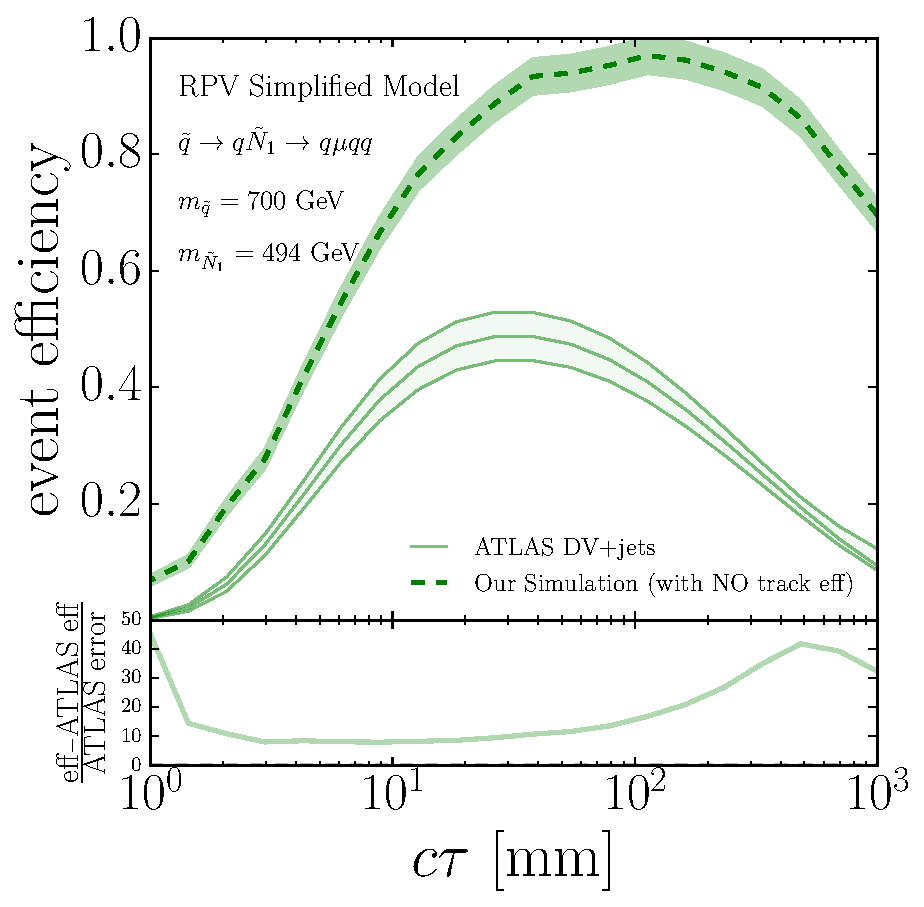
\includegraphics[width=0.49\textwidth,angle=0]{ch5-figures/effVsCtau_RPVValidation_NoTrkEff.pdf}
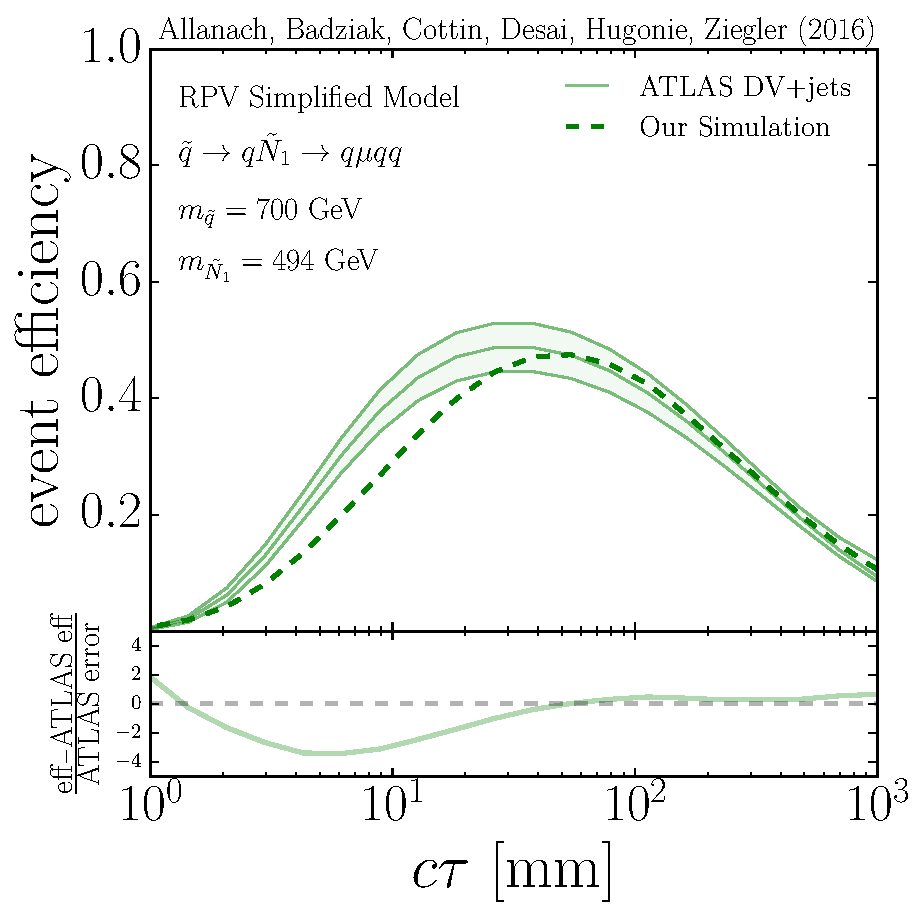
\includegraphics[width=0.49\textwidth,angle=0]{ch5-figures/effVsCtau_RPVValidation.pdf}
\end{center}
\caption{Validation of the DV + jets search for the ATLAS benchmark of a simplified RPV model
  with a 700 GeV squark decaying to a neutralino, $\tilde q \rightarrow q (\tilde N_{1} \rightarrow \mu \bar u d)$ \label{fig:trkeff}. {\bf{Left:}} without any tracking efficiency. {\bf{Right:}} with a tracking efficiency function given by equation~\ref{eqn:trkeff}, taken from Ref~\cite{Allanach:2016pam}.}
\end{figure}

\vskip 0.1in
\noindent {\bf Lessons learned}
\vskip 0.1in

With a larger and more diverse set of signal benchmarks, the prospects for reinterpretation are better. For example, the ATLAS analysis examined in Ref.~\cite{ATLAS-CONF-2013-092} only showed limits for three signal model benchmark points for which efficiencies were shown, making it challenging to find a benchmark whose kinematics matched the desired signal models for the reinterpretations of other models (for example, in Ref.~\cite{Cui:2014twa}). Because the efficiencies and limits were shown for either a high-mass, low-boost LLP \emph{or} a low-mass, high-boost LLP, this made it more challenging to reinterpret the results for other types of kinematics.

The new parametrized efficiencies presented by ATLAS in Ref.~\cite{SUSY-2016-08} are extremely useful. They constitute an optimal efficiency map for recasting these type of analyses, as they can by applied in a straightforward way to truth-level quantities. Before this information was made public, efficiency tables (for vertex-level efficiency) in terms of $r_\mathrm{DV}$ were only available for few channels and for a single benchmark. It was not clear how to translate this information to other channels, or to parent particles of a different mass. In this case, a functional parametrization for track efficiency was needed (as derived in Ref.~\cite{Allanach:2016pam}) to be able to reproduce the experimental results. Finding this kind of parametrization is not easy, as it needs to be validated across different benchmarks. For example, Ref.~\cite{Allanach:2016pam} found that fitting only one benchmark did not correctly reproduce the event-level efficiency curve for any of the others.



